\documentclass[conference]{IEEEtran}
\IEEEoverridecommandlockouts
% The preceding line is only needed to identify funding in the first footnote. If that is unneeded, please comment it out.
\usepackage{cite}
\usepackage{amsmath,amssymb,amsfonts}
\usepackage{algorithmic}
\usepackage{graphicx}
\usepackage{multicol}
\usepackage{minted}
\usepackage{textcomp}
\usepackage{xcolor}

\def\BibTeX{{\rm B\kern-.05em{\sc i\kern-.025em b}\kern-.08em
    T\kern-.1667em\lower.7ex\hbox{E}\kern-.125emX}}
\begin{document}
\title{Paper Reading of \textit{Phosphor: Illuminating Dynamic Data Flow in Commodity JVMs}, and its application on flaky tests}

\author{\IEEEauthorblockN{Yiwei Yang}
    \IEEEauthorblockA{\textit{School of Information Science and Technology} \\
        \textit{ShanghaiTech University}\\
        Shanghai, China \\
        yangyw@shanghaitech.edu.cn}
}

\maketitle

\begin{abstract}
    With the flaky test \cite{b6}, that in continuous unit test/ fuzzing/ regression tests integration, some of them may pass and not pass from time to time because of (non)order dependencies variables, , is getting more severe for concurrent programs, we have to come up with a software engineering method to identify and fix.
    Other than \cite{b2}, a tool to identify the flaky test by checking original order passes, running different thread order configurations, and finally rerunning the truncated failing order and truncated original order. We could use a previous Dynamic Taint Analysis on order dependent variables to get a possible order dependent variable to automate the debugging process.
    Phosphor \cite{b1} is a taint tracking system based on bytecode modifications. The object of taint tracking is the tracking of specific data variables. can be used to find brittle test,
\end{abstract}

\begin{IEEEkeywords}
    JVM, program analysis, dynamic taint analysis, flaky test
\end{IEEEkeywords}

\section{Paper Summary}
\subsection{Basic principles of dynamic taint analysis}
Taint analysis can be abstracted into a triplet $\langle sources, sinks, processor\rangle$ where source represents the direct introduction of untrusted data or confidential data into the system, sink represents direct generation of security-sensitive operations and processor the entire process of data transmission and processing.

For taint convergence points, they can be broadly classified conceptually into 3 categories.
\begin{figure}[htbp]
    \centering
    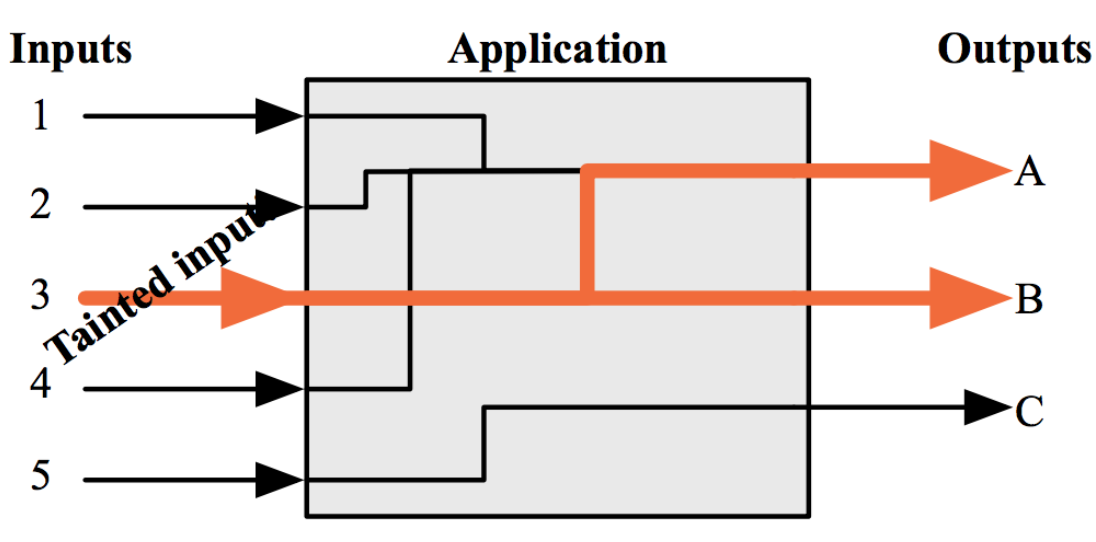
\includegraphics[width=0.6\columnwidth]{./taint.png}
    \caption{Dynamic Taint Analysis}
\end{figure}
\begin{enumerate}
    \item Use heuristic strategies for tagging. e.g. mark network data transmission.
    \item Manually mark sources and aggregation points depending on the API or important data types called by the specific application. e.g. filesystem access.
    \item Automatically identify and tag taint sources and aggregation points using statistical or machine learning techniques. \cite{b7}
\end{enumerate}
Phosphor first taints the variable, cast processor on java bytecode to propagate the taint.
\begin{enumerate}
    \item Leverages benefits of interpreter-based approaches (information about variables) but fully portably
    \item Instruments all byte code that runs in the JVM (including the JRE API) to track taint tags
          \begin{enumerate}
              \item Add a variable for each variable
              \item Adds propagation logic
          \end{enumerate}
          \begin{figure}[htbp]
              \centering
              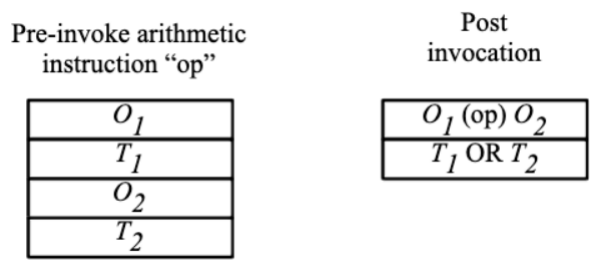
\includegraphics[width=0.6\columnwidth]{./stack_code.png}
              \caption{Stack Code Propagation logic}
          \end{figure}
\end{enumerate}

\subsection{Connection with Flaky tests}
When a developer commits code to a repository, tests are run to see if the changes have broken any functionality. Every new test failure would ideally be due to the developer's most recent modifications, allowing the developer to focus on fixing these problems. Unfortunately, some failures are due to flaky tests rather than the most recent updates. When executed on the same version of the code, a flaky test can pass or fail non-deterministically, flaky tests may also pass when they should have failed. Flaky testing are unavoidable in most modern applications. Take, for example, a Google system test that involves loading a website with an ad inserted in it. If the ad serving system becomes overburdened and is unable to deliver an ad within a reasonable amount of time, the test may be sent a page without ads. In this situation, the test runner might not be able to tell the difference between a malfunctioning ad server (which may not be serving ads to any clients) and a functional ad server that just dropped the request.
Test order dependencies are closely linked to flakiness or tests that can fail unexpectedly if run in a different order. This early work (PraDet \cite{b8}) looked at how to quickly isolate tests to avoid flakiness and how to exactly discover which tests depend on one other, allowing developers to detect which orderings will result in flakiness.
\section{Positive}
\begin{enumerate}
    \item The framework is generic and easy to use. You can embed any type of DTA to your project and report as a maven plugin.
    \item Give a sound and complete propagation rule for all Java ASM.
          \begin{figure}[htbp]
              \centering
              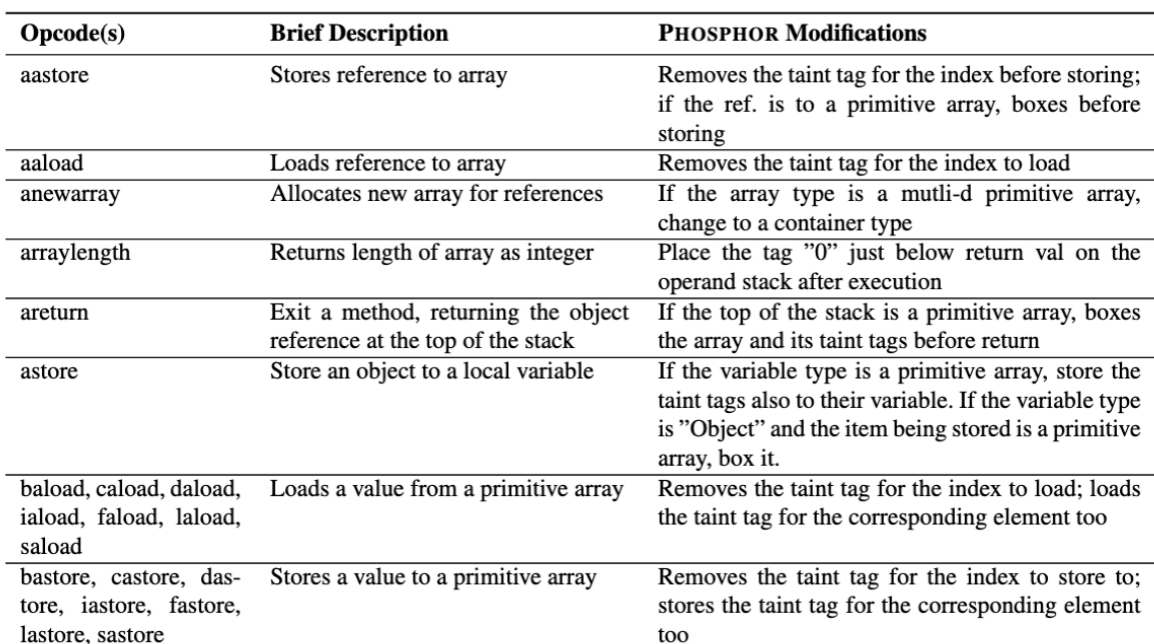
\includegraphics[width=0.6\columnwidth]{./jvm_array.png}
              \caption{JVM propagation logic array part}
          \end{figure}
    \item Use taint tag storages
          \begin{figure}[htbp]
              \centering
              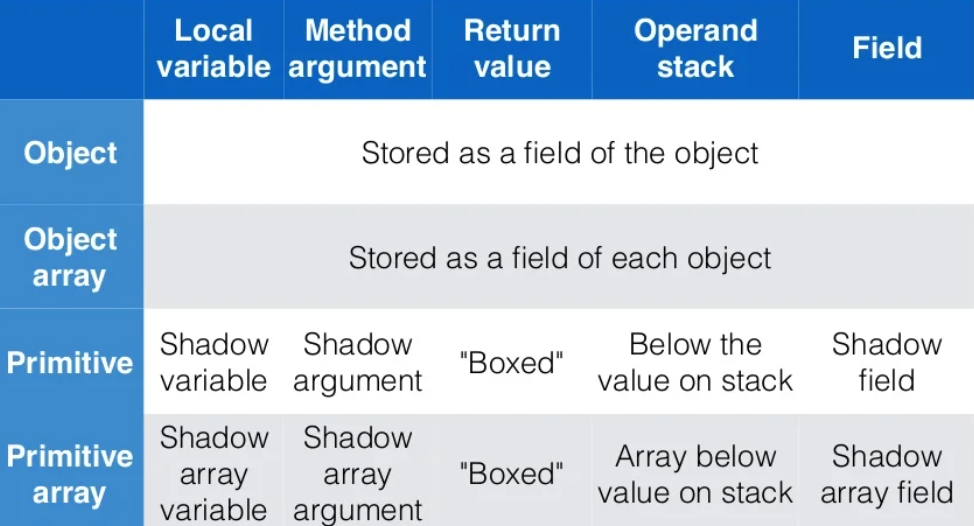
\includegraphics[width=0.6\columnwidth]{./taint_storage.png}
              \caption{Phosphor Taint Tag Storage}
          \end{figure}
\end{enumerate}
\section{Negative}
\begin{enumerate}
    \item For specific purposes, because of the overhead of framework instrumentation, the effectiveness may not be as good as the specifically designed cases. For example, PraDet \cite{b5} introduced before is 10 times faster in finding order dependent variables.
    \item Java ASM debugging is harder than you think. And the reference is not fruitful.
\end{enumerate}
\section{Soundness}
The primary concern of dynamic implicit flow analysis is how to determine the range of statements to be marked under taint control conditions. Since the dynamic execution trajectory does not reflect the control dependencies among the instructions being executed, most of the current research uses offline static analysis to assist in determining the scope of implicit flow marking in dynamic taint propagation.

\subsection{Taint propagation analysis}
\subsubsection{Explicit Flow Analysis}
Analyze how taint marks propagate with "data dependencies" between variables in the program.
\setlength{\columnsep}{-2cm}
\begin{multicols}{2}
    \begin{minted}[mathescape,escapeinside=||]{java}
void explicit_foo (){
 int a = |\colorbox{green}{source()}|;
 int b = |\colorbox{green}{source()}|;
 int x, y;
 |\colorbox{green}{x}| = a * 2;
 |\colorbox{green}{y}| = b + 4;
 |\colorbox{red}{sink(x)}|;
 |\colorbox{red}{sink(y)}|;
}

\end{minted}
    \begin{minted}[mathescape,escapeinside=||]{java}
void implicit_foo (){
String X = |\colorbox{green}{source()}|;
String Y = new String();
for (int i=0; i<X.length(); i++) {
 int |\colorbox{blue}{x}| = (int) X.charAt(i);
 int y = 0;
 for (int j=0; j<x; j++) |\colorbox{green}{y}|=y+1;
 |\colorbox{green}{Y}| = Y + (char) y;
 |\colorbox{red}{sink(Y)}|;
}
\end{minted}
\end{multicols}
% \setlength{\columnsep}{0cm}
a and b are marked as taint sources by the predefined taint source function source.
Assume that a and b are given the taint tags taint\_a and taint\_b, respectively.

Since the variable x in row 5 has a direct data dependency on variable a and the variable y in row 6 has a direct data dependency on variable b, explicit stream analysis will propagate the taint markers taint\_a and taint\_b to the variable x in row 5 and the variable y in row 6, respectively.
Since x and y can reach the taint convergence point in rows 7 and 8, respectively, at the taint convergence point, we can follow a predefined strategy to draw conclusions, such as the information leakage problem of the code shown above.
\subsubsection{Implicit Flow Analysis}
Analyze how taint marks propagate with "control dependencies" between variables in the program, that is, how taint marks propagate from conditional instructions to the statements they control.

Variable X is a tainted string type variable. There is no direct or indirect data dependency (explicit flow relationship) between variable Y and variable X, but the tainted token on X can be implicitly propagated to Y through the control dependency.
Specifically, the outer loop controlled by the loop condition in line 4 sequentially takes out each character in X, converts it to an integer and assigns it to variable x. The inner loop controlled by the loop condition in line 7 then assigns the value of x to y in a cumulative manner, and finally the outer loop passes y to Y one by one.
In the end, the value of Y in line 12 is the same as the value of X. The program has an information leakage problem.
\section{Significance}
The Phosphor framework has been widely used in \cite{b11}
\begin{enumerate}
 \item Unknown Vulnerability Detection, like finding concurrent bugs \cite{b10}.
 \item Automatic Input Filter Generation. Forward symbolic execution can be used to automate the generation of filter.
 \item Malware Analysis.
 \item Test Case Generation.
 \end{enumerate}

\section{Novelty}
\subsection{Applied DTA on instrumented nearly all JVM}
It defined a full processor on JVM byte code and instrumented the Java standard library for harmless processing. The tainted data may pass through the harmless processing module during the process of dissemination. The harmless processing module means that after the tainted data is processed by this module, the data itself no longer carries sensitive information or the operation against the data will no longer be harmful to the system. In other words, tainted data can be removed after passing through the hold harmless module.
Proper use of harmless processing can reduce the number of taint marks in the system, improve the efficiency of taint analysis, and avoid the problem of inaccurate analysis results due to taint proliferation.

it's applied to three completely different JVMs (in addition to the two versions of Oracle’s HotSpot and Open-JDK’s IcedTea, plus the Dalvik DVM).
\subsection{Applied DTA on Android}
Phosphor can be utilized on Android java apps with additional instrumented system calls. \cite{b10} Although PHOSPHOR was built for the JVM, we realized that it could also be used with Android's own virtual machine, the Dalvik Virtual Machine (DVM). Almost all Android applications are written in Java, which is subsequently compiled to Java byte code and translated into dex, the DVM's byte code format. We may apply PHOSPHOR to Android and the DVM by putting taint propagation logic in the intermediate Java byte code before it is translated to dex, because it executes a translated form of Java byte code and PHOSPHOR operates at the byte code level.
\subsection{A generic scalable programming framework}
All other DTA related work can be written into the codebase, e.g. brittle tests \cite{b5}.
\section{Verifiability}
\subsection{Experiment}
The paper cast experiments on \texttt{DroidBench}. 64 tests were all passed,and we can see array-heavy benchmarks is not as performant as TaintDroid\cite{b10}.
\begin{figure}[htbp]
    \centering
    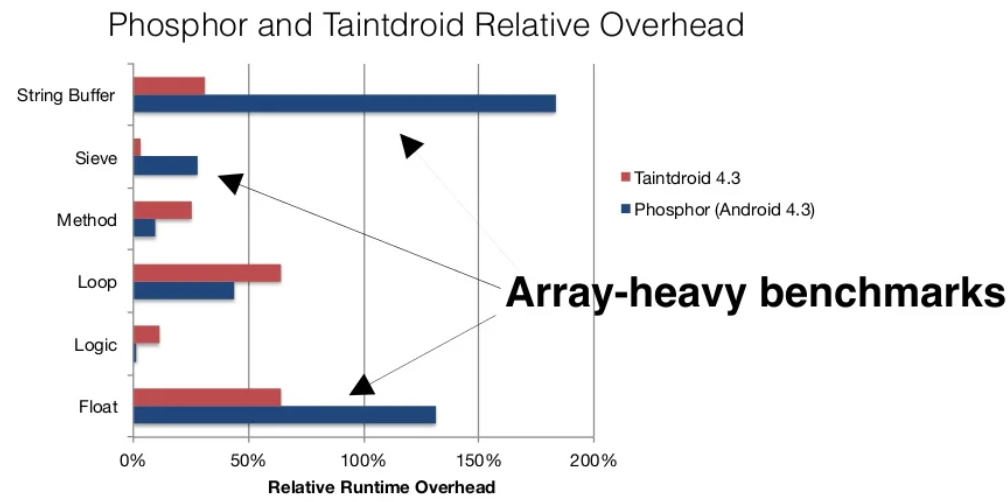
\includegraphics[width=0.6\columnwidth]{./taintdroid.png}
    \caption{DroidBench}
\end{figure}
\subsection{The taint source and propagation analysis}
This paper \cite{b12} provides a symbolic execution analysis on the taint source and prpagaiton analysis to identify the soundness and precision of jvm bytecode.
\begin{figure}[htbp]
    \centering
    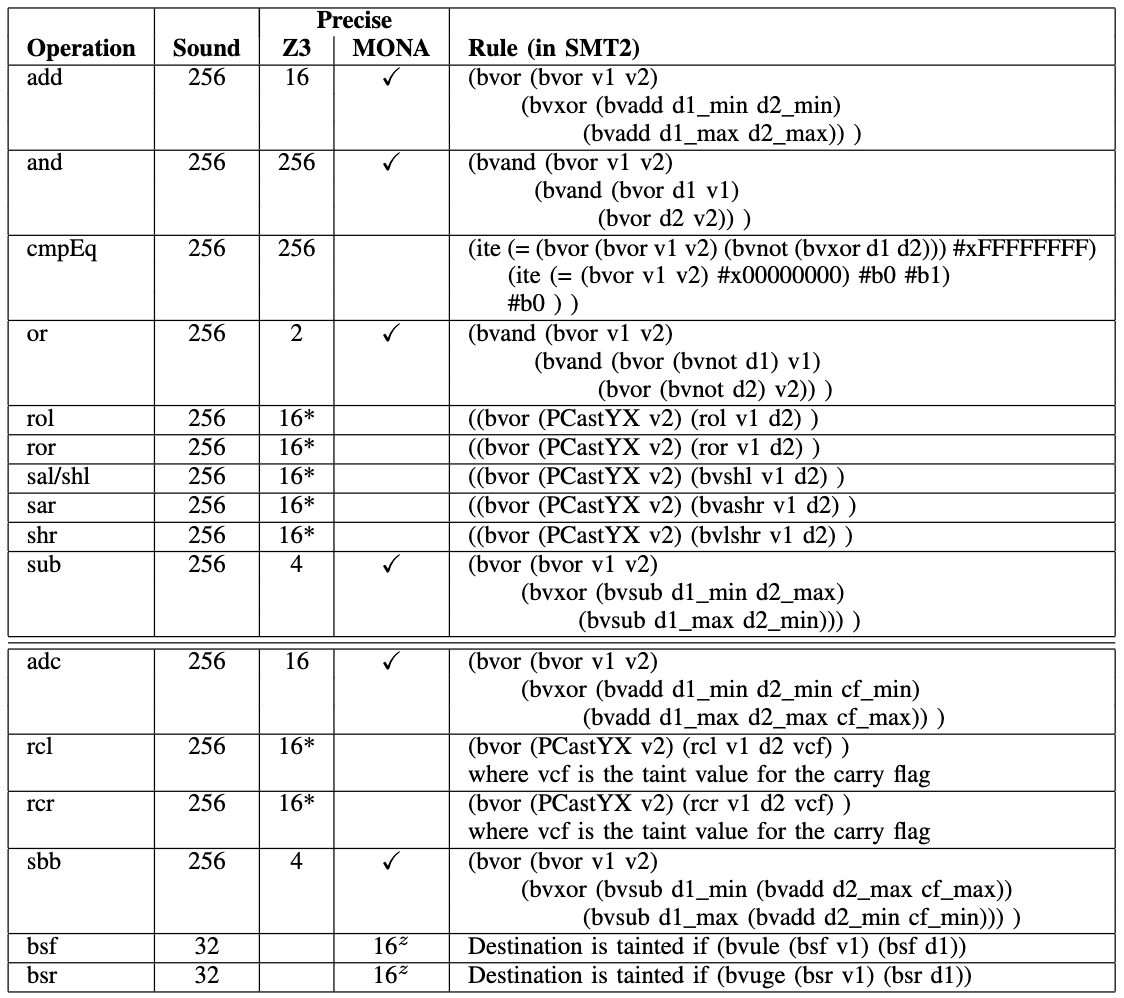
\includegraphics[width=\columnwidth]{./z3.png}
    \caption{Sok}
\end{figure}

\section{Connection}
\subsection{Compared with previous DTA that failed to maintain soundness and precision.}
All of them associate tags with data, then propagate the tags, and they are not portable
\begin{enumerate}
    \item Operating System modifications
    \item Language interpreter modifications
    \item Source code modifications
    \item Binary instrumentation of applications
\end{enumerate}

\subsection{Compared with the newer published PraDet \cite{b8}} It has 10x slower performance. PraDet applies the jvm heap DTA and instrument the stdlib more aggressively. As for tests, the PraDet will execute the different manifestation order by its analysed possible order and do refinement on order check to get the real order. However, we indeed can use Phosphor to implement the PraDet.


\subsection{Compared with other symbolic execution tool called Java PathFinder doing order dependent finding variables.}
"Polluter tests" are tests that change (or "pollute") the common state among tests in a test suite. Finding these tests is critical since the sequence in which the tests in the test suite are run can result in various test outcomes. Previously, the PolDet technique was presented for locating polluter tests in JUnittest runs on a normal Java Virtual Machine (JVM). Given that JavaPathFinder (JPF) provides desirable infrastructure support, such as methodically investigating thread schedules, re-implementing techniques like PolDet in JPF is a worthwhile endeavour. \cite{b4} 

\section{Brainstorming}

\subsection{Use in Order Dependent flaky tests}
Flaky tests are a common problem in software testing, that the failure of test is non-deterministic. The flaky tests are usually order dependent. e.g.
\begin{minted}[mathescape]{java}
    class D {
      static Mutable2 staticField; // this will not be changed
      static {
        staticField = new Mutable2();
        staticField.next = new Mutable2();
      }
    }
    class Mutable2 { Mutable2 next /* = null */;}
    class BasicFlakyAssertionTest {
      // should be null
      void t1() {System.out.println(D.staticField.next.next); }
      // passes if run after t2 but fails if run before
      void t3() {assertNotNull(D.staticField.next.next); }
      void t2() {D.staticField.next.next = new Mutable2(); }
    }
    \end{minted}
The solution to identify the above case is pretty simple in phosphor.
\begin{enumerate}
\item Taint all mutable field, array, primitive variable
\item propogate as in the Phosphor
\item if 2 paths meet in the assertion's variable there's OD.
\end{enumerate}
\subsection{Refinement of the effectiveness}
Basically, if you get more information from the analysis, the less information you need to cache during runtime.
\begin{enumerate}
\item Use JPF - symbolic execution for getting runtime type info/deterministic path to minimize the processor state
\item Can utilize prediction-based taint tracking (propagation) approach, and design statistical experiments to observe some special properties of load and store instructions in the CPU instruction stream.
\item Can transform dynamic taint analysis into a problem handled by deferred exceptions.
\end{enumerate}

\begin{thebibliography}{00}
    \bibitem{b1} BELL, Jonathan; KAISER, Gail. Phosphor: Illuminating dynamic data flow in commodity jvms. Acm Sigplan Notices, 2014, 49.10: 83-101.
    \bibitem{b2} W. Lam, R. Oei, A. Shi, D. Marinov and T. Xie, "iDFlakies: A Framework for Detecting and Partially Classifying Flaky Tests," 2019 12th IEEE Conference on Software Testing, Validation and Verification (ICST), 2019, pp. 312-322, doi: 10.1109/ICST.2019.00038.
    \bibitem{b3} ANAND, Saswat; PĂSĂREANU, Corina S.; VISSER, Willem. JPF–SE: A symbolic execution extension to java pathfinder. In: International conference on tools and algorithms for the construction and analysis of systems. Springer, Berlin, Heidelberg, 2007. p. 134-138.
    \bibitem{b4} YI, Pu, et al. Finding Polluter Tests Using Java PathFinder. ACM SIGSOFT Software Engineering Notes, 2021, 46.3: 37-41.
    \bibitem{b5} HUO, Chen; CLAUSE, James. Improving oracle quality by detecting brittle assertions and unused inputs in tests. In: Proceedings of the 22nd ACM SIGSOFT International Symposium on Foundations of Software Engineering. 2014. p. 621-631.
    \bibitem{b6} Wing Lam, Stefan Winter, Anjiang Wei, Tao Xie, Darko Marinov, and Jonathan Bell. 2020. A large-scale longitudinal study of flaky tests. Proc. ACM Program. Lang. 4, OOPSLA, Article 202 (November 2020), 29 pages.
    \bibitem{b7} SHE, Dongdong, et al. Neutaint: Efficient dynamic taint analysis with neural networks. In: 2020 IEEE Symposium on Security and Privacy (SP). IEEE, 2020. p. 1527-1543.
    \bibitem{b8} GAMBI, Alessio; BELL, Jonathan; ZELLER, Andreas. Practical test dependency detection. In: 2018 IEEE 11th International Conference on Software Testing, Verification and Validation (ICST). IEEE, 2018. p. 1-11.
    \bibitem{b9} Fang-Hsiang Su, J. Bell, G. Kaiser and S. Sethumadhavan, "Identifying functionally similar code in complex codebases," 2016 IEEE 24th International Conference on Program Comprehension (ICPC), 2016, pp. 1-10, doi: 10.1109/ICPC.2016.7503720.
    \bibitem{b10} SUN, Mingshen; WEI, Tao; LUI, John CS. Taintart: A practical multi-level information-flow tracking system for android runtime. In: Proceedings of the 2016 ACM SIGSAC Conference on Computer and Communications Security. 2016. p. 331-342.
    \bibitem{b11} SCHWARTZ, Edward J.; AVGERINOS, Thanassis; BRUMLEY, David. All you ever wanted to know about dynamic taint analysis and forward symbolic execution (but might have been afraid to ask). In: 2010 IEEE symposium on Security and privacy. IEEE, 2010. p. 317-331.
    \bibitem{b12} YAN, Lok Kwong; YIN, Heng. SoK: On the Soundness and Precision of Dynamic Taint Analysis. Formal. Taint, 2017, 2017: 1-15.
\end{thebibliography}
\end{document}
